\chapter{The Architecture of Reality: Foundations of EDC}
\label{ch:foundations}

\begin{center}
\textit{Mathematical Foundations of the Geometric Arena in Elastic Diffusive Cosmology}
\end{center}

\vspace{1em}

\noindent This chapter establishes the mathematical foundations of EDC. We begin with cognitive preparation --- analogies that help the reader overcome the intuitive barriers to higher-dimensional thinking. We then proceed to rigorous mathematics, stating our assumptions explicitly and deriving consequences through standard techniques.

Our central thesis is ambitious: \textbf{the properties of spacetime, quantum mechanics, and matter emerge from the geometry of a 5-dimensional manifold}. We proceed axiomatically. Where we make conjectures beyond established mathematics, we label them clearly.

% ═══════════════════════════════════════════════════════════════════════════════
% SECTION 2.1: COGNITIVE PREPARATION
% ═══════════════════════════════════════════════════════════════════════════════

\section{Cognitive Preparation: Overcoming Our Dimensional Blindness}
\label{sec:cognitive_preparation}

Before we can define the physics of a new paradigm, we must confront a biological obstacle. The crisis of modern physics is not merely in our equations; it is rooted in our brains.

Evolution has wired the human neocortex for survival in a strictly 3-dimensional Euclidean environment. We understand concepts like ``up,'' ``down,'' ``left,'' and ``right'' because these vectors enabled us to hunt and avoid predators. However, our cognitive hardware possesses a fundamental limitation that makes us blind to the true nature of reality: \textbf{The Dimensional Ceiling}.

Our minds can mathematically manipulate $n$ dimensions, but can visualize only three. We are like pattern-matching engines hard-coded for 3D rendering; any input from the 4th or 5th spatial dimension is automatically compressed, projected, or rejected by our brains as ``counterintuitive.'' This is why quantum mechanics appears ``strange'' to us---not because nature is strange, but because our perspective is incomplete.

To understand \textit{Elastic Diffusive Cosmology} (EDC), you must consciously bypass these evolutionary defaults. You must accept that what you see is only a shadow---a projection---of a far richer structure.

\subsection{The Hardware Limitation}

Our brains are pattern-matching engines optimized for 3D survival. We can see a cube, rotate it mentally, count its faces. This happens effortlessly because evolution wired us for three dimensions.

But try to visualize a 4D hypercube---a tesseract. Your mind cannot hold it. You see rotating projections, wire-frame shadows---anything but the actual 4D object. This is not a failure of imagination; it is a \textbf{hardware constraint}.

When physicists encounter phenomena that suggest 5D geometry---entanglement, vacuum energy, dark matter---they face the same constraint. Rather than accept that reality extends beyond 3D, they:

\begin{itemize}
    \item Declare phenomena ``acausal'' (quantum nonlocality)
    \item Add mysterious postulates (wavefunction collapse)
    \item Invent invisible entities (dark matter particles)
\end{itemize}

\textbf{EDC requires you to override this bias.} Accept that what you perceive is a projection---a shadow---of a richer 5D structure. Your intuition is not wrong; it is simply incomplete.

\subsection{The Second Barrier: Time as Flow}

Beyond the dimensional ceiling, we face another hardwired limitation: \textbf{the perception of time as flow}.

We experience time as:

\begin{itemize}
    \item \textbf{Duration}: The interval needed to move from point A to point B
    \item \textbf{Waiting}: The subjective sense of something ``taking time''
    \item \textbf{Arrow}: The irreversible march from past to future
\end{itemize}

But Einstein's relativity treats time as a \textit{static dimension}---just another coordinate like length. This is the ``block universe'' view: all moments (past, present, future) exist simultaneously in 4D spacetime.

Most people find this philosophically uncomfortable. Why does time \textit{feel} like flow if it's really just geometry?

\textbf{EDC Resolution:}

Time is \textit{not} a dimension. Time is a \textbf{process measure}---specifically, the rate of energy diffusion through the Plenum.

What we call ``the passage of time'' is the propagation rate of disturbances through the viscous Bulk. When energy diffuses slowly (high viscosity), time ``passes slowly.'' When energy diffuses quickly, time ``passes quickly.''

\begin{equation}
\Delta t \sim \frac{\ell^2}{\eta_{\text{bulk}}/\rho_{\text{bulk}}} \quad \text{(diffusion timescale)}
\end{equation}

This is why:

\begin{itemize}
    \item Time has an \textbf{arrow} (diffusion is irreversible; entropy increases)
    \item Space does \textbf{not} have an arrow (you can move left or right freely)
    \item Time dilation occurs near massive objects (membrane curvature affects diffusion rates)
\end{itemize}

Time is fundamentally different from space because it measures \textit{change in the medium}, not position in the medium.

\subsection{The Illusion of Uncertainty: The Cylinder Analogy}

Why does the nature of light seem paradoxical to us? Why does Heisenberg's principle claim we cannot simultaneously know the exact position and exact momentum of a quantum object? Standard physics teaches us that nature is fundamentally uncertain at that scale.

EDC offers a different answer: \textbf{Nature is perfectly determined, but we are looking at a projection.}

Imagine a simple three-dimensional object: \textbf{a Cylinder}.

Now imagine you are a 2D being living on a flat wall, able to see only the shadow that cylinder casts on your wall.

\begin{enumerate}
    \item \textbf{Projection A (Side View):} If light falls from the side, the cylinder's shadow on the wall is a \textbf{Rectangle}. The 2D being measures this as ``Wavelength'' (Momentum).
    
    \item \textbf{Projection B (Head-On View):} If we rotate the cylinder 90 degrees, its shadow becomes a \textbf{Circle}. The 2D being measures this as ``Position of a point.''
\end{enumerate}

2D scientists would endlessly argue: \textit{``Is the object fundamentally rectangular or circular?''}

Heisenberg's principle in their world would state: \textit{``It is impossible to simultaneously see the rectangularity and circularity of an object.''}

This is true for a 2D projection, but it is false for the 3D object. The cylinder possesses attributes of both rectangle and circle simultaneously, but those attributes are encoded in a higher dimension that the 2D observer cannot encompass in a single view.

In our universe, what we call a \textbf{photon} is a quantum of the 5D electromagnetic field $A_B$. When we ``measure'' it, we force this 5D excitation to project onto our 3D membrane. In the process of projection, we lose part of the information.

\textbf{Uncertainty is not an ontological property of the universe; it is a consequence of information loss during geometric projection.}

\begin{figure}[h]
\centering
\includegraphics[width=0.75\textwidth]{figures/cylinder_projections.png}
\caption{\textbf{The Illusion of Uncertainty.} A 3D cylinder projects different shapes onto 2D surfaces depending on viewing angle. Projection A (side view) reveals a rectangle---analogous to measuring wavelength/momentum. Projection B (head-on view) reveals a circle---analogous to measuring position. A 2D observer cannot see both projections simultaneously, creating apparent ``complementarity.'' In EDC, photons are quanta of the 5D field $A_B$; measurements force 3D projections, losing information. Heisenberg uncertainty is not ontological---it is geometric information loss.}
\label{fig:cylinder}
\end{figure}

\subsection{Topological Blind Spot: The Ant on the Möbius Strip}

To understand how thoroughly we are trapped in our own perception, we must understand the difference between \textit{dimension} and \textit{topology}.

Imagine an ant walking along a long strip of paper.

The ant is effectively a 2D being. It understands only two axes: \textbf{X} (forward-backward) and \textbf{Y} (left-right). For the ant, the world is flat. It knows there is a ``top'' surface it walks on, and it can theoretically imagine there is a ``bottom'' side, but it cannot reach the bottom without drilling a hole through the paper (which would be a cataclysmic event for the ant).

Now we, from our 3D perspective, do something simple: we take the ends of the strip, twist one end by \textbf{180 degrees}, and connect them. We have created a \textbf{Möbius strip}.

What happened to the ant?

The ant continues walking. It walks straight along the X axis. Eventually, it will complete a full circuit and return to where it started---but it will find itself on what it previously called the ``bottom side.'' If it continues walking, it will return to the starting point again.

\textbf{The crucial insight is this: The ant does not know that we twisted the strip.}

The twist occurred in the \textbf{Z axis} (height)---a dimension the ant cannot see or conceive.

\begin{itemize}
    \item To the ant, the strip has simply become \textbf{longer} (an infinite loop)
    \item It still perceives only X and Y
    \item It has no idea that ``two sides'' have merged into one
\end{itemize}

The ant experiences the \textit{consequences} of the higher dimension (path infinity, side merging) but cannot see the \textit{cause} (the twist in 3D). To understand what happened, the ant would have to ``exit'' the strip---which is impossible.

\textbf{We are in the same position.} We live in 3D space (our strip) which may be bent, twisted, or immersed in the 5D Plenum. We see the consequences of that bending (quantum entanglement, nonlocality), but we interpret them as ``strange physics'' within our 3D strip, rather than as simple geometry in a higher dimension.

This insight leads us to a crucial question: If we cannot ``exit'' the strip to see the higher dimension, can we detect something that \textit{enters} our strip from outside?

\begin{figure}[h]
\centering
\includegraphics[width=0.65\textwidth]{figures/mobius_strip.png}
\caption{\textbf{Topological Blindness.} A 2D ant walking on a Möbius strip experiences both ``sides'' as a single connected surface but cannot perceive the twist in the 3rd dimension. The ant detects consequences (infinite path, side merging) without seeing the cause (geometric twist). Similarly, we observe quantum entanglement and nonlocality (consequences) without perceiving the 5D geometric connections (cause). The twist is invisible to membrane-bound observers.}
\label{fig:mobius}
\end{figure}

\subsection{The Ontology of Light: The Flux Event}

Here we arrive at the resolution of a century-old paradox: How can a particle be a wave? This paradox vanishes if we view our universe as a surface upon which something falls from that ``invisible dimension.''

Imagine our universe as the calm surface of a lake (the Membrane). Above it, in the air (the Plenum)---that dimension the ant knows nothing about---a raindrop forms in a cloud.

\subsubsection{The Journey of the Drop}

\textbf{1. The Descent (Travel Through the Bulk):} 

While the drop falls through the air, it is a coherent packet of mass and energy. However, to flat creatures (ants) living \textit{on} the surface of the water, this drop does not exist. It is ``outside'' their reality. It occupies no coordinates in their space and time.

\textbf{2. The Impact (Interaction):} 

The drop strikes the surface of the lake. This is the moment we call ``photon detection.''

\subsubsection{Duality as a Consequence of Perspective}

The impact manifests in two ways:

\begin{itemize}
    \item It appears as a \textbf{WAVE} when we observe the \textbf{consequences of impact} on the elastic membrane (propagation of vibrations, interference). This is the ``side view'' of the cylinder.
    
    \item It appears as a \textbf{PARTICLE} when we observe the \textbf{impact location} (energy transfer at a point). This is the ``head-on view'' of the cylinder.
\end{itemize}

The creature on the surface asks: \textit{``Was it a wave or a particle? It traveled as a wave but hit as a particle!''}

The answer is: \textbf{It was neither.} It was a drop falling from a higher dimension.

In EDC, a photon is not a particle traveling \textit{along} the membrane. It is a \textbf{flux event}---an energy packet falling \textit{from} the Bulk onto the membrane. We see the splash (detection) and the ripples (interference), but we miss the drop's journey through the Bulk because our eyes cannot look ``up'' into the 5th dimension.

\begin{figure}[h]
\centering
\includegraphics[width=0.85\textwidth]{figures/raindrop_flux_event.png}
\caption{\textbf{The Flux Event: Resolving Wave-Particle Duality.} A photon originates in the Bulk (analogous to a raindrop in air above a lake surface). \textit{(1) Descent:} The drop falls through the Bulk---invisible to membrane observers. \textit{(2) Impact:} The drop strikes the membrane (flux event)---this is ``photon detection.'' \textit{(3) Ripples:} The impact creates spreading waves on the membrane surface---this is interference. Surface observers see both particle (localized splash) and wave (ripples), but miss the drop's 5D journey. The photon is neither particle nor wave---it is a boundary-crossing event.}
\label{fig:raindrop}
\end{figure}

\subsection{Beyond Dimensions: The Physics of Manifestation}

We have established that the photon is not a 3D particle traveling along the membrane, but a 5D flux event---a coherent structure in the Plenum that interacts with our membrane. But we must now address a deeper question:

\textit{What does it mean for something to exist in 5 dimensions?}

The naive answer would be: ``Take our familiar 3D space (x, y, z), add two more coordinates ($w_1$, $w_2$), and now you have 5D.'' This is mathematically correct but \textbf{physically misleading}.

\textbf{More dimensions does not mean more coordinates. More dimensions means new physics---new modes of manifestation.}

\subsubsection{The Fallacy of ``Just Add Coordinates''}

Consider again our 2D ant on the Möbius strip. We tell the ant: ``Your world is not truly 2D. There is a third dimension---height (Z)---that you cannot perceive.''

The ant might respond: ``Fine. So my position is now (X, Y, Z) instead of just (X, Y). What changes?''

\textbf{Everything changes.}

The ant does not simply gain a new coordinate. The ant gains:

\begin{itemize}
    \item The ability for paths to \textbf{cross without intersecting} (overpasses in 3D)
    \item The possibility of \textbf{rotation} that reverses left/right (the Möbius twist)
    \item The existence of \textbf{enclosed volumes} (caves, which are impossible in pure 2D)
\end{itemize}

These are not just ``extra numbers.'' These are \textbf{qualitatively new phenomena} that do not exist in 2D at all.

\subsubsection{5D Physics: New Manifestations, Not Just New Axes}

When we say the photon is a 5D object, we do not mean it has five position coordinates that we could measure if we had the right instrument. We mean:

\textbf{The photon's interaction with 3D structures produces phenomena that cannot be explained by 3D physics alone.}

Specifically, a 5D flux event crossing into our 3D membrane can manifest in \textit{fundamentally different ways} depending on the \textbf{geometry of the 3D structure it encounters}.

\subsubsection{Two Types of 3D Structures}

Our membrane is not empty. It contains structures---obstacles, detectors, lattices---that are themselves confined to 3 spatial dimensions. When the 5D photon encounters these structures, the interaction depends critically on their geometry.

\paragraph{Type 1: Thin Barriers (Wave Manifestation)}

Consider a metal plate with two narrow slits---our classic double-slit apparatus. This barrier has:

\begin{itemize}
    \item \textbf{3D structure:} Defined positions in (x, y, z)
    \item \textbf{Thickness:} A few millimeters in our 3D space
    \item \textbf{But in 5D?} The barrier is \textit{infinitely thin}---it exists only on the membrane $\Sigma$, with no extension into the Bulk direction $w$ or the compact dimension $\xi$
\end{itemize}

\paragraph{Type 2: Deep Absorbers (Particle Manifestation)}

Now consider a different structure: a CCD pixel in a camera sensor, or an electron in an atom that can absorb the photon.

This structure has:

\begin{itemize}
    \item \textbf{3D structure:} A localized region in (x, y, z)
    \item \textbf{But in 5D?} The absorber creates a ``potential well'' that extends into the $w$-direction through its distortion of the Plenum
\end{itemize}

%═══════════════════════════════════════════════════════════════════════════════
\subsection{Resolution of the Wave-Particle Duality: The Surfer and the Wake}
\label{sec:double_slit}
%═══════════════════════════════════════════════════════════════════════════════

The double-slit experiment is often cited as the ultimate mystery of quantum mechanics. How can a single particle pass through two slits simultaneously? Standard quantum mechanics answers with a metaphysical abstraction: the particle exists as a superposition of probabilities until observed.

\textbf{EDC offers a strictly geometric, realist resolution.}

\subsubsection{The Particle and the Wake}

In EDC, we must distinguish two entities that are always together but fundamentally different:

\begin{itemize}
    \item \textbf{The Particle (The Surfer):} The topological defect itself---a ``knot'' on the membrane. It is \textit{local}. It has a definite position.
    \item \textbf{The Field (The Wake):} As the defect moves through the Bulk, it generates elastic disturbances in the $\Phi$ and $A_B$ fields. These waves propagate through the extra dimensions ($w$ and $\xi$) at the speed of the medium.
\end{itemize}

\begin{figure}[h]
\centering
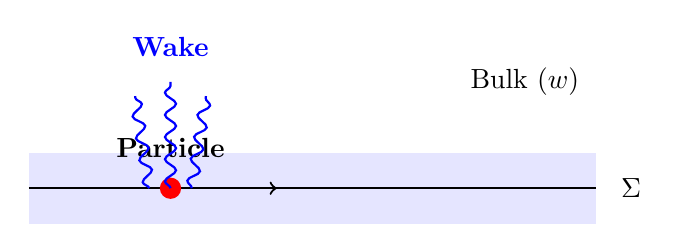
\begin{tikzpicture}[scale=0.9]
    % Membrane
    \fill[blue!10] (-4,-0.5) rectangle (4,0.5);
    \draw[thick] (-4,0) -- (4,0);
    \node at (4.5,0) {$\Sigma$};
    
    % Particle (surfer)
    \fill[red] (-2,0) circle (0.15);
    \node[above] at (-2,0.3) {\textbf{Particle}};
    
    % Wake (waves extending into bulk)
    \draw[blue, thick, decorate, decoration={snake, amplitude=2pt, segment length=8pt}] 
        (-2,0) -- (-2,1.5);
    \draw[blue, thick, decorate, decoration={snake, amplitude=2pt, segment length=8pt}] 
        (-2.3,0) -- (-2.5,1.3);
    \draw[blue, thick, decorate, decoration={snake, amplitude=2pt, segment length=8pt}] 
        (-1.7,0) -- (-1.5,1.3);
    \node[blue] at (-2,2) {\textbf{Wake}};
    
    % Bulk label
    \node at (3,1.5) {Bulk ($w$)};
    
    % Arrow showing motion
    \draw[->, thick] (-1.5,0) -- (-0.5,0);
\end{tikzpicture}
\caption{\textbf{The Surfer and the Wake.} A particle (topological defect) is localized on the membrane $\Sigma$, but it generates waves that extend into the Bulk. The particle ``surfs'' on its own wake.}
\label{fig:surfer_wake}
\end{figure}

\subsubsection{Mechanism of Interference}

When an electron approaches the double-slit barrier:

\begin{enumerate}
    \item \textbf{The Particle (Defect)} passes through \textit{only one} slit. There is no paradox of location---the particle is always local.
    
    \item \textbf{The Bulk Wave (Wake)}, being a non-local deformation of the surrounding Plenum, passes through \textit{both} slits.
    
    \item On the far side of the barrier, the waves from the two slits collide, creating an interference pattern of high and low geometric pressure (constructive and destructive interference).
    
    \item The particle, emerging from its single slit, encounters this turbulent geometric sea. It is guided (``piloted'') by the interference pattern of its own wake.
\end{enumerate}

The particle does not randomly choose a path; it \textbf{surfs the geometric contours of the Bulk}. We detect the particle at a specific point (where it hits the screen), but the statistical distribution of many such impacts reveals the wave pattern of the guiding field.

\begin{tcolorbox}[colback=blue!5,colframe=blue!60!black,title=Derivation: The Geometric Origin of de Broglie Wavelength]
We can now derive the famous de Broglie relation $\lambda = h/p$ from pure geometry.

The action of the membrane is quantized by the geometric scale:
\begin{equation}
\hbar_{\text{geom}} = \frac{\sigma R_\xi^3}{c}
\end{equation}

A particle with momentum $p$ corresponds to a wave mode with wavenumber $k$ in the Bulk. The resonance condition between the particle's motion and the Bulk elastic waves is:
\begin{equation}
p = \hbar_{\text{geom}} \cdot k = \frac{h}{\lambda}
\end{equation}

Thus, the ``matter wave'' wavelength $\lambda$ is simply the beat frequency between the particle's scan velocity and the natural vibration modes of the membrane thickness $R_\xi$.

\textbf{The de Broglie relation is not mysterious---it is geometry.}
\end{tcolorbox}

\subsubsection{The ``Collapse'' Explanation}

Why does placing a detector at the slit destroy the interference pattern?

In EDC, a detector is not a passive observer. It is a massive collection of defects (atoms). To detect the electron, the detector must \textit{interact} with it via the electromagnetic field ($A_B$).

This interaction creates a new, chaotic ``splash'' in the Bulk fluid, scrambling the delicate interference pattern coming from the other slit. The pilot wave is disrupted, and the electron reverts to simple ballistic motion.

\textbf{No metaphysics is required---only hydrodynamics.}

\begin{tcolorbox}[colback=green!5,colframe=green!60!black,title=EDC vs. Standard Quantum Mechanics]
\begin{center}
\begin{tabular}{|p{4cm}|p{4cm}|p{4cm}|}
\hline
\textbf{Question} & \textbf{Standard QM} & \textbf{EDC} \\
\hline
What is the particle? & Probability amplitude & Topological defect (local) \\
\hline
What passes through both slits? & The particle itself (superposition) & The wake (Bulk waves) \\
\hline
Why interference? & ``Wave function'' & Pilot wave in Plenum \\
\hline
Why does detection destroy pattern? & ``Collapse'' (undefined) & Detector creates chaotic splash \\
\hline
Is the particle ever delocalized? & Yes (superposition) & \textbf{No}---always local \\
\hline
\end{tabular}
\end{center}
\end{tcolorbox}

\subsubsection{Experimental Support: Couder's Walking Droplets}

This is not mere speculation. In 2005, Yves Couder and Emmanuel Fort demonstrated that oil droplets bouncing on a vibrating fluid surface exhibit \textit{exactly this behavior}:

\begin{itemize}
    \item The droplet (particle) bounces on the surface
    \item Each bounce creates waves that spread across the fluid
    \item The droplet ``surfs'' on its own waves
    \item In a double-slit geometry, single droplets produce interference patterns!
\end{itemize}

These ``walking droplets'' are a macroscopic analog of EDC's pilot-wave mechanism. The quantum world is not fundamentally different from classical hydrodynamics---it is simply operating in higher dimensions.

%═══════════════════════════════════════════════════════════════════════════════
\subsection{Quantum Entanglement: The 5D Connection}
\label{subsec:entanglement}
%═══════════════════════════════════════════════════════════════════════════════

Entanglement is often called ``the strangest feature of quantum mechanics''---Einstein's ``spooky action at a distance.'' Two particles, separated by any distance, remain perfectly correlated. Measure one, and you instantly know the state of the other.

Standard quantum mechanics offers no mechanism. It simply states that the joint wavefunction cannot be factored: $\psi_{AB} \neq \psi_A \otimes \psi_B$. The correlation is a brute mathematical fact.

\textbf{EDC provides a geometric mechanism.}

\begin{tcolorbox}[colback=blue!5,colframe=blue!60!black,title=\textbf{Entanglement: Connection Through the Bulk}]

When two particles are generated in an entangled state, they are not two separate geometric defects. They are \textbf{two endpoints of a single, continuous 5D structure}---a ``U-tube'' or vortex loop extending into the Bulk.

\begin{itemize}
    \item \textbf{On the Membrane (3D):} The particles appear separated by distance $\Delta x$ (potentially kilometers or light-years).
    
    \item \textbf{In the Bulk (5D):} The geometric distance along the connecting structure is minimal---they are joined at the ``base'' of the U-tube.
\end{itemize}

Measurement of particle A induces a torsional disturbance along this 5D structure, which is \textit{instantly} felt at endpoint B. The correlation is instantaneous because, \textbf{topologically, A and B are parts of the same object}.

\vspace{0.3cm}
\textbf{Conclusion:} Entanglement is not a signal sent across space. It is the vibration of a shared geometric root in the extra dimension.

\vspace{0.3cm}
\begin{center}
\textit{Information does not travel \textbf{across} space; it travels \textbf{beneath} it.}
\end{center}

\vspace{0.3cm}
\textbf{Connection to ER = EPR:} This 5D geometric connection is the concrete realization of the Maldacena-Susskind ``ER = EPR'' conjecture (2013). In EDC, quantum entanglement (EPR) \textit{is} a microscopic wormhole (Einstein-Rosen bridge) through the Bulk. The conjecture becomes a theorem.
\end{tcolorbox}

\subsubsection{The Iceberg Analogy}

Imagine two icebergs floating miles apart on the ocean surface. A 2D observer (confined to the surface) sees them as separate objects. They wonder: ``How is it that when I push one, the other moves instantly?''

A diver (3D observer) sees the truth: beneath the surface, the two ``icebergs'' are peaks of a single massive underwater mountain. They are connected at the base.

There is no magic. There is only hidden geometry.

\begin{figure}[h]
\centering
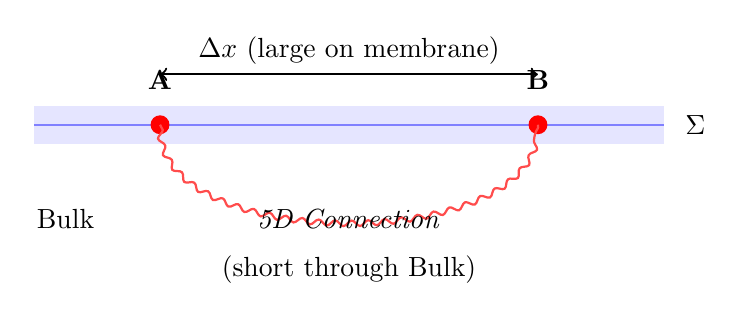
\begin{tikzpicture}[scale=0.8]
    % Membrane surface
    \fill[blue!10] (-5,-0.3) rectangle (5,0.3);
    \draw[thick, blue!50] (-5,0) -- (5,0);
    \node at (5.5,0) {$\Sigma$};
    
    % Particle A
    \fill[red] (-3,0) circle (0.15);
    \node[above] at (-3,0.4) {\textbf{A}};
    
    % Particle B
    \fill[red] (3,0) circle (0.15);
    \node[above] at (3,0.4) {\textbf{B}};
    
    % U-tube in bulk
    \draw[thick, red!70, decorate, decoration={snake, amplitude=1pt, segment length=6pt}] 
        (-3,0) .. controls (-3,-2) and (3,-2) .. (3,0);
    
    % Distance labels
    \draw[<->, thick] (-3,0.8) -- (3,0.8);
    \node[above] at (0,0.8) {$\Delta x$ (large on membrane)};
    
    % Bulk label
    \node at (0,-1.5) {\textit{5D Connection}};
    \node at (0,-2.3) {(short through Bulk)};
    
    % Bulk region
    \node at (-4.5,-1.5) {Bulk};
\end{tikzpicture}
\caption{\textbf{Entanglement as 5D Connection.} Particles A and B appear separated on the membrane $\Sigma$, but are connected through a U-tube structure in the Bulk. Measurement of A disturbs the entire structure, instantly affecting B. The ``spooky action'' is simply the vibration of a shared geometric object.}
\label{fig:entanglement}
\end{figure}

\subsubsection{Compatibility with Bell's Theorem}

Bell's theorem (1964) proves that no theory with \textit{local} hidden variables can reproduce quantum correlations. Experiments have confirmed Bell inequality violations to $>100\sigma$.

Does EDC violate Bell's theorem? \textbf{No.}

EDC is a \textbf{non-local geometric theory}:
\begin{itemize}
    \item The hidden variable is the 5D structure connecting the particles
    \item This structure is \textit{not local} in 3D space---it extends through the Bulk
    \item Bell's theorem excludes \textit{local} hidden variables; it does not exclude \textit{geometric} connections through extra dimensions
\end{itemize}

EDC survives Bell's test because the ``hidden variable'' is the topology of the 5D manifold itself---something that appears non-local when projected onto 3D.

\begin{tcolorbox}[colback=yellow!5,colframe=orange!60!black,title=\textbf{The Einstein-Bohr Reconciliation}]
The Bohr-Einstein debates (1927--1935) centered on whether quantum mechanics was ``complete.'' Einstein insisted reality must be local and deterministic. Bohr insisted the quantum formalism was final.

\textbf{EDC reconciles both positions:}
\begin{itemize}
    \item \textbf{Bohr was right:} The phenomenon \textit{is} non-local in 3D. Bell's theorem is valid. No 3D local hidden variable theory can reproduce quantum correlations.
    
    \item \textbf{Einstein was right:} Reality \textit{is} local---in 5D. The ``spooky action'' is an artifact of dimensional projection. In the full geometry, everything is causally connected through the Bulk.
\end{itemize}

There is no contradiction. They were both correct---just in different dimensions.
\end{tcolorbox}

\begin{tcolorbox}[colback=green!5,colframe=green!60!black,title=The Quantum Trilogy: EDC Explanations]
\begin{center}
\begin{tabular}{|l|l|l|}
\hline
\textbf{Phenomenon} & \textbf{Standard QM} & \textbf{EDC} \\
\hline
Wave-Particle Duality & Superposition (mystery) & Surfer \& Wake \\
\hline
Wavefunction Collapse & Undefined & Detector splash in Bulk \\
\hline
Entanglement & Spooky action (no mechanism) & 5D U-tube connection \\
\hline
\end{tabular}
\end{center}

\vspace{0.3cm}
\textit{All three ``mysteries'' of quantum mechanics are geometric consequences of our membrane being embedded in a higher-dimensional Bulk.}
\end{tcolorbox}

\subsubsection{Micro vs Macro Wormholes: Why We Can't Travel Through}

If entanglement is a wormhole, why can't we use it for faster-than-light travel or communication?

The answer lies in membrane tension $\sigma$.

\textbf{Micro-wormholes (quantum entanglement):}
\begin{itemize}
    \item Particle-scale U-tubes are \textit{natural}---they form spontaneously when particles interact
    \item The energy cost is minimal (comparable to particle rest masses)
    \item The universe is \textit{filled} with these micro-connections---they are the ``stitches'' holding spacetime together
\end{itemize}

\textbf{Macro-wormholes (sci-fi traversable tunnels):}
\begin{itemize}
    \item To create a human-sized wormhole, you must bend the membrane until it ``touches itself'' through the Bulk
    \item The membrane tension $\sigma \sim 10^{18}$ J/m$^2$ resists this deformation \textit{violently}
    \item Energy required: $E \sim \sigma \cdot A \sim 10^{18} \times 1 \text{ m}^2 = 10^{18}$ J (equivalent to $\sim 10^{11}$ kg of mass-energy)
\end{itemize}

\textbf{Conclusion:} Micro-wormholes are free; macro-wormholes cost more energy than a star. This is why quantum entanglement is ubiquitous, but traversable wormholes remain science fiction.

\subsection{Energy Transfer: Three Fates of the Photon}

When a 5D photon enters our universe (crosses the membrane), its energy must go somewhere. There are three possibilities, each determined by the type of 3D structure it encounters:

\subsubsection{Fate 1: Complete Absorption (Heat)}

The photon encounters a material particle---an electron in a metal, an atom in a crystal lattice. The absorber has a deep 5D potential well. The photon's energy is:

\begin{itemize}
    \item Localized at a single point $(x_0, y_0, z_0)$
    \item Converted entirely into kinetic energy (the electron recoils)
    \item Dissipated as heat (random thermal motion)
\end{itemize}

\textbf{Manifestation:} Pure particle. The photon ``died'' at a single location.

\textbf{Example:} Sunlight warming your skin. Each photon is absorbed by a molecule, increasing its vibrational energy. No interference, no wave behavior---just localized energy packets hitting one molecule at a time.

\subsubsection{Fate 2: Electron Ejection (Photoelectric Effect)}

A higher-energy photon strikes an atom. If the photon's energy exceeds the electron's binding energy:

\begin{itemize}
    \item The photon's 5D field excitation collapses into the atom's potential well (deep in $w$)
    \item The electron absorbs the energy and escapes the atom
    \item The photon ceases to exist; an electron is ejected
\end{itemize}

\textbf{Manifestation:} Pure particle. Einstein's 1905 insight: light delivers energy in discrete packets, not continuous waves.

\textbf{But in EDC:} The ``packet'' is not a fundamental property of light. It is the consequence of the photon's 5D field excitation being forced to localize by the atom's deep potential well (which extends into $w$-space). The atom, by its geometry, conditioned the photon to manifest as a particle.

\subsubsection{Fate 3: Diffraction (Wave Behavior)}

The photon encounters a periodic structure---a crystal lattice, a diffraction grating. The structure has:

\begin{itemize}
    \item Regular spacing: $d \sim$ Angstroms (for X-rays) or micrometers (for visible light)
    \item Thin geometry in $w$ (the crystal is a membrane-bound structure)
\end{itemize}

The photon's 5D trajectory interacts with \textit{multiple atoms simultaneously}. Because the structure is thin in $w$, the photon maintains its 5D coherence. The membrane vibrates in a diffraction pattern---Bragg peaks, interference fringes.

\textbf{Manifestation:} Pure wave.

\textbf{The crystal lattice, by its physical properties (periodic spacing, thin $w$-geometry), conditioned the 5D photon to manifest as a wave.}

\subsubsection{The Atomic Lattice as a Natural Double-Slit}

This leads to a profound realization:

\textbf{X-ray crystallography is a double-slit experiment at the atomic scale.}

When we fire X-rays at a crystal:

\begin{itemize}
    \item The periodic array of atoms acts as a 3D diffraction grating
    \item The crystal is thin in $w$ (atomic-scale structures do not extend far into the Bulk)
    \item The X-ray photon (5D soliton) maintains coherence across multiple atoms
    \item The result: Bragg diffraction---a clear interference pattern
\end{itemize}

\textbf{The atoms did not ``measure'' the photon. They provided a thin periodic structure that allowed wave manifestation.}

If we replaced the crystal with a \textit{thick absorber} (say, a block of lead), the photons would be absorbed individually---particle manifestation. No diffraction. The lead's deep $w$-geometry forces particle behavior.

\subsection{The Invisible Messenger: Why Time Does Not Exist for the Photon}

Here we arrive at one of the deepest physical truths we often overlook:

\textbf{We have never seen a photon in flight.}

We cannot ``catch'' a photon to examine it and then release it onward. The only way to detect a photon is to destroy it (absorb it) on the retina of an eye or a camera sensor.

Until that moment of measurement (and the type of structure it encounters), we have absolutely no information about that photon in our universe.

Photons are everywhere around us, all the time, but they travel as 5D entities---``ghosts'' that possess attributes of the space they come from (the Bulk), not the space they apparently traverse (the Membrane).

Because of this, \textbf{time does not exist for them.}

When we look at a distant galaxy, we say the light traveled for a billion years. But for the photon, the journey was instantaneous. It did not ``swim'' through our membrane, struggling against its viscosity and friction (which we experience as the passage of time). It leaped through the Bulk.

Only when we capture it on a telescope mirror---at the moment of its death---do our brains and instruments reconstruct the ``distance'' and calculate the ``time'' that supposedly passed. Time is an artifact of our perception, a post-processing construction of an event that, for the photon itself, was a timeless 5D jump.

% ═══════════════════════════════════════════════════════════════════════════════
% THE HOLOGRAPHIC RECONSTRUCTION PRINCIPLE
% ═══════════════════════════════════════════════════════════════════════════════

\subsection{The Holographic Reconstruction Principle}
\label{sec:holographic_principle}

Before stating our postulates, we must address a foundational methodological question that will recur throughout this book:

\textit{If we cannot escape the 3D membrane to directly observe the 5D Plenum, how can we learn anything about it?}

The answer defines the epistemological foundation of EDC.

\begin{tcolorbox}[colback=blue!5,colframe=blue!70!black,title=\textbf{The Platonic Foundation}]
For two millennia, Plato's Cave has served as philosophical metaphor: prisoners see shadows on a wall and mistake them for reality. The shadows are \textit{projections} of higher-dimensional objects they cannot directly perceive.

\textbf{EDC makes this metaphor into physics.}

We are observers confined to a 3D membrane. Everything we measure---particles, forces, masses---are ``shadows'': projections of 5D geometric structures onto our lower-dimensional surface. The Standard Model is our precise catalog of these shadows.
\end{tcolorbox}

But here is the crucial insight: \textbf{shadows contain information about the objects that cast them}.

A sphere passing through a 2D plane creates a circular shadow that grows, reaches maximum, then shrinks. A Flatland physicist measuring this shadow cannot directly deduce ``sphere''---but by analyzing shadow properties (radius, rate of change), they can \textit{reconstruct} the 3D object that caused it.

\textbf{This is exactly what EDC does with the Standard Model.}

\begin{tcolorbox}[colback=green!5,colframe=green!60!black,title=The Reconstruction Principle]
\textbf{Statement:} Standard Model observations are not ``inputs'' that EDC borrows. They are \textit{boundary conditions}---empirical data about the 3D shadow that constrain and reveal the 5D geometry.

\textbf{Methodology:}
\begin{enumerate}
    \item We observe physical phenomena in our 3D world
    \item We propose these arise from higher-dimensional geometry
    \item We derive relationships between observed quantities
    \item Agreement validates the higher-dimensional interpretation
\end{enumerate}

\textbf{Consequence:} When EDC uses observed physical properties---this is not ``borrowing parameters.'' It is \textit{reading the geometric signature of the Bulk from the surface boundary}.
\end{tcolorbox}

To make this concrete, consider how a Flatland physicist might work:

\begin{itemize}
    \item \textbf{Shadow observation:} A circular shadow appears, grows to maximum radius $R$, then shrinks and vanishes
    \item \textbf{3D interpretation:} This pattern is consistent with a sphere of radius $R$ passing through the plane
    \item \textbf{Test:} If it's truly a sphere, the shadow area should follow $A(t) = \pi(R^2 - z(t)^2)$---and it does!
\end{itemize}

The Flatland physicist did not ``derive'' that there must be a sphere. But by proposing a sphere and checking that shadow measurements match, they confirmed the 3D interpretation. The shadow data became evidence for the higher-dimensional object.

\textit{This is exactly what EDC does---not only with particles, but with all of physics.}

Throughout this book, we will show that when we interpret our 3D observations as projections of 5D geometry, remarkable consistencies emerge across all domains: quantum mechanics, gravity, cosmology, and particle physics. Phenomena that appear unrelated in 3D reveal themselves as different facets of the same 5D structure.

\textit{The shadows match the geometry. The geometry explains the shadows.}

This principle---using 3D observations to reconstruct higher-dimensional structure---will guide us throughout this book. We are not prisoners who can escape Plato's Cave. But we are prisoners who can reason about the fire from the patterns of light on our wall.

\subsection{Why Five Dimensions? The Principle of Minimal Extension}
\label{sec:why_5D}

The reader may ask: \textit{Why propose exactly 5 dimensions? Why not 6, or 7, or 11 as in M-theory?}

Our choice is guided by a principle we call \textbf{minimal extension}:

\begin{tcolorbox}[colback=gray!10,colframe=gray!60!black,title=The Principle of Minimal Extension]
When existing theory proves insufficient, extend it by the \textit{smallest increment} that might resolve the problems. If that increment fails, extend further. Do not assume more structure than necessary.
\end{tcolorbox}

Consider what we already know:
\begin{itemize}
    \item \textbf{3 spatial dimensions} $(x, y, z)$ --- established by everyday experience
    \item \textbf{1 time dimension} $(t)$ --- established by Einstein's relativity
\end{itemize}

This gives us 4 dimensions (3+1 spacetime), which successfully describes electromagnetism, special relativity, and much of physics. But 4D is \textit{not enough}: quantum mechanics remains mysterious, gravity resists unification, dark matter and dark energy lack explanation.

The next logical step is \textbf{5D}: one additional dimension beyond what we know works.

\begin{center}
\textit{If 5D fails to explain the phenomena, we will acknowledge failure and try 6D.\\
If 5D succeeds, we will have found the minimal extension that works.}
\end{center}

\subsubsection{What Does a ``New Dimension'' Mean?}

A common misconception must be addressed: \textbf{a new dimension does not necessarily mean another direction like left-right, up-down, or forward-backward.}

Einstein's great insight was precisely this. When he introduced time as the fourth dimension, he did not mean that time is ``another spatial direction.'' Time is fundamentally different from space:
\begin{itemize}
    \item We can move freely in spatial directions; we cannot move backward in time
    \item Spatial distances add by Pythagoras ($ds^2 = dx^2 + dy^2 + dz^2$); spacetime intervals subtract time ($ds^2 = dx^2 + dy^2 + dz^2 - c^2dt^2$)
    \item Time is \textit{orthogonal} to space in a geometric sense, yet manifests as something qualitatively different---duration, causality, entropy
\end{itemize}

The lesson: \textbf{each new dimension represents a new mode of physical manifestation}, not merely ``more room.''

In EDC, the fifth dimension $\xi$ is likewise not ``another spatial direction.'' Just as Einstein's time dimension enabled new physics (relativity, causality, the connection between mass and energy), our fifth dimension will enable new physics---phenomena that appear mysterious when viewed from 3D alone.

We do not yet specify what $\xi$ ``is'' in physical terms. That understanding will emerge as we develop the theory. For now, the key insight is methodological:

\begin{center}
\textit{The question is not ``where does the 5th dimension point?''\\but rather ``what new phenomena does it make possible?''}
\end{center}

As this book will demonstrate, 5D proves to be \textit{sufficient}. The additional dimension---interpreted as a compact spatial dimension through which energy flows---resolves the crises of modern physics without requiring the elaborate structures of string theory (which invokes 10 or 11 dimensions).

This is not a claim that higher dimensions do not exist. It is a methodological choice: \textbf{start simple, extend only as needed}. The success of EDC vindicates this conservative approach.

\subsection{The Stage of the Universe: Two Postulates}

After we have removed cognitive illusions about the nature of light, we can lay the physical foundations of Elastic Diffusive Cosmology. EDC rests on two geometric postulates.

\begin{tcolorbox}[colback=blue!5,colframe=blue!70,title=Postulate 1: The Plenum (The Bulk)]
The universe is a 5-dimensional continuum filled with an energetic fluid. This fluid is not empty space; it is a dynamic medium of high energy density. It is the reservoir from which all energy (light) in our world originates.

We characterize the Plenum by two fundamental properties:

\begin{itemize}
    \item \textbf{Energy density} $\rho_{\text{bulk}}$ (mass per unit 5D volume)
    \item \textbf{Viscosity} $\eta_{\text{bulk}}$ (resistance to flow)
\end{itemize}

\textbf{Terminology:} We use ``Plenum'' and ``Bulk'' interchangeably. ``Plenum'' emphasizes the fluid's energetic fullness (from Latin \textit{plenus} = full), while ``Bulk'' emphasizes its role as the higher-dimensional container. Throughout this book, we capitalize both terms when referring to this specific 5D medium.
\end{tcolorbox}

\begin{tcolorbox}[colback=blue!5,colframe=blue!70,title=Postulate 2: The Membrane (The Brane)]
Our physical reality---the space we see around us---is a 3-dimensional elastic sheet (phase boundary) floating in the Plenum. The light we see consists of transverse vibrations of this membrane caused by flux events from the Plenum.

We characterize the Membrane by two fundamental properties:

\begin{itemize}
    \item \textbf{Surface tension} $\sigma$ (energy per unit area; units J/m$^2$)
    \item \textbf{Surface density} $\rho_s$ (mass per unit area)
\end{itemize}
\end{tcolorbox}

\begin{tcolorbox}[colback=blue!5,colframe=blue!70,title=Postulate 3: The Plenum Energy Density]
In addition to $\sigma$ and $R_\xi$, we introduce a third macroscopic parameter: the Plenum energy density $\rho_{\text{Plenum}}$, taken as a \textbf{fundamental parameter} of the theory.

\textbf{Physical interpretation:} The Plenum is not empty space with occasional fluctuations. It is a \textit{maximally dense} energetic medium. Matter (vortices on the membrane) exists as localized \textit{deficits}---``holes'' or ``bubbles''---within this dense background.

\textbf{Role in the theory:} In the full EDC program, $\rho_{\text{Plenum}}$ sets the gravitational coupling scale through the dynamics of Plenum flow. In this edition, $\rho_{\text{Plenum}}$ is treated as a fundamental model parameter; its relation to $G$ is developed in Chapter~7 (consistency checks) and Chapter~8 (emergent-metric framework).

\textbf{Order of magnitude (a posteriori comparison):} For orientation, we note that the numerical value of $\rho_{\text{Plenum}}$ will later be compared to the conventional Planck density $\rho_{\text{Planck}} \equiv c^7/(\hbar G^2) \approx 5 \times 10^{96}$ J/m$^3$. This comparison is made \textit{after} deriving consequences---it does not enter the postulate itself.
\end{tcolorbox}

\vspace{0.5em}
\noindent\textbf{Summary of the Three Pillars:}
\begin{center}
\small
\begin{tabular}{|l|l|l|}
\hline
\textbf{Parameter} & \textbf{Role} & \textbf{Status} \\
\hline
$\sigma$ (surface tension) & sets $\hbar_{\text{geom}}$ (Ch.~6) & to be constrained \\
$R_\xi$ (compact radius) & sets $U(1)$ scale (Ch.~3,6) & to be constrained \\
$\rho_{\text{Plenum}}$ (Plenum density) & sets $G$ coupling scale & fundamental parameter \\
\hline
\end{tabular}
\end{center}
\normalsize

\textbf{We do not live in empty space. We live on the surface of an ocean of energy.}

\newpage

% ═══════════════════════════════════════════════════════════════════════════════
% SECTION 2.2: THE GEOMETRIC ARENA
% ═══════════════════════════════════════════════════════════════════════════════

\section{The Geometric Arena}
\label{sec:geometric_arena}

Having prepared the mind for higher-dimensional thinking, we now establish the mathematical stage on which physics unfolds. In EDC, this stage is not the familiar 4D spacetime of Einstein, but a richer 5-dimensional structure we call the \textbf{Bulk}.

\subsection{The Bulk Manifold}
\label{subsec:bulk_manifold}

We posit that physical reality is embedded in a 5-dimensional manifold $\mathcal{M}_5$ with coordinates:
\begin{equation}
X^A = (w, x^1, x^2, x^3, \xi) = (w, x, y, z, \xi)
\end{equation}
where:
\begin{itemize}
    \item $w$: \textbf{Bulk Time} --- the fundamental temporal coordinate of the Bulk, providing causal structure
    \item $x, y, z$: Three spatial dimensions (our observable universe, the Membrane $\Sigma$)
    \item $\xi$: A compact internal dimension with topology $S^1$ and radius $R_\xi$
\end{itemize}

The coordinate $\xi$ is periodic:
\begin{equation}
\xi \sim \xi + 2\pi R_\xi
\end{equation}

This seemingly technical detail --- that $\xi$ wraps around on itself like a circle --- will prove crucial. It is the geometric origin of \textit{electric charge quantization}, as we shall see in Section~\ref{sec:electric_charge}.

\vspace{0.5em}
\noindent\textbf{A note on terminology}: In the cognitive preparation above, we used intuitive language like ``the Bulk is timeless'' or ``static.'' We now recognize that this was imprecise. The Bulk possesses its own temporal dimension $w$; what is emergent on the Membrane is not time itself, but rather \textit{our perceived time} $t$, which arises from the Membrane's motion through the Bulk. This distinction is subtle but important: the Bulk has causal structure, but we experience only a slice of it.

\subsection{The Bulk Metric}
\label{subsec:bulk_metric}

The geometry of the Bulk is specified by its metric --- the rule for measuring distances and angles. We equip $\mathcal{M}_5$ with a pseudo-Riemannian metric of Lorentzian signature $(-,+,+,+,+)$:
\begin{equation}
\boxed{ds^2_{\text{Bulk}} = -dw^2 + dx^2 + dy^2 + dz^2 + R_\xi^2 \, d\xi^2}
\label{eq:bulk_metric_ch2}
\end{equation}

In matrix form, the metric tensor is:
\begin{equation}
G_{AB} = \begin{pmatrix}
-1 & 0 & 0 & 0 & 0 \\
0 & 1 & 0 & 0 & 0 \\
0 & 0 & 1 & 0 & 0 \\
0 & 0 & 0 & 1 & 0 \\
0 & 0 & 0 & 0 & R_\xi^2
\end{pmatrix}
\end{equation}

\textbf{Critical point}: The coordinate $w$ carries a \textbf{negative signature}. This single minus sign is not an arbitrary choice but a \textit{necessity} for causal structure. The negative sign identifies $w$ as the temporal dimension, enabling:
\begin{itemize}
    \item Distinction between past and future (causal ordering)
    \item Wave propagation (hyperbolic field equations)
    \item Light cones and null geodesics
\end{itemize}

Without this minus sign, the Bulk would be a static, frozen geometry with no dynamics --- a mathematical construct devoid of physics.

\subsection{The Membrane and Emergent Time}
\label{subsec:membrane_time}

Our observable 3D universe (the Membrane $\Sigma$) is a hypersurface that moves through the Bulk. Picture a sheet of paper sliding through a book: the paper is our universe, the book is the Bulk, and the act of sliding is the passage of time.

Mathematically, the Membrane's trajectory is parameterized by:
\begin{equation}
w(t) = v_{\text{scan}} \cdot t
\end{equation}
where $t$ is the \textbf{emergent time} parameter experienced by membrane-bound observers (us!), and $v_{\text{scan}}$ is the scanning velocity --- how fast the Membrane moves through the Bulk.

\textbf{Physical interpretation}: What we perceive as ``time'' ($t$) is the projection of fundamental Bulk-time ($w$) onto the Membrane. The Membrane ``sails'' through the Bulk at constant velocity $v_{\text{scan}}$. Every moment of our experience corresponds to a different slice of the eternal Bulk.

\subsection{Derivation of the Induced Metric via Pullback}
\label{subsec:pullback}

A natural question arises: if we live on a moving Membrane embedded in a 5D Bulk, what geometry do \textit{we} experience? The answer comes from the mathematical operation called the \textbf{pullback}, which projects the Bulk metric onto the Membrane.

\begin{tcolorbox}[colback=blue!5,colframe=blue!70!black,title=Conceptual Visualization: The Röntgen Universe]
Before diving into the mathematics, consider a helpful analogy.

A medical X-ray shines through a complex 3D body (bones, organs, tissues) and captures a 2D projection on a film. The film shows darker spots where dense structures block the radiation.

\begin{itemize}
    \item \textbf{The 5D Bulk} is the body---rich, structured, and complex
    \item \textbf{Our 3D Membrane} is the X-ray film
    \item \textbf{The ``particles'' we measure} are the darker spots---projections of 5D knots and vortices
    \item \textbf{The pullback operation} is the X-ray process itself---it determines \textit{how} 5D structure gets imprinted onto 3D
\end{itemize}

A heavier particle like the Z boson appears as a ``denser'' spot than the electron---more 5D structure is being projected. The mathematics below makes this precise.

\textit{We are living inside the X-ray image.}
\end{tcolorbox}

Let the membrane embedding be $X^A(x^\mu)$ where $x^\mu = (t, x, y, z)$ are the 4D spacetime coordinates on the membrane. The induced metric is given by:
\begin{equation}
g_{\mu\nu} = G_{AB} \frac{\partial X^A}{\partial x^\mu} \frac{\partial X^B}{\partial x^\nu}
\end{equation}

For a membrane at fixed $\xi = \xi_0$ moving through the Bulk with $w = v_{\text{scan}} t$, the embedding is:
\begin{equation}
X^A(t, x, y, z) = (v_{\text{scan}} \, t, \, x, \, y, \, z, \, \xi_0)
\end{equation}

Computing the partial derivatives:
\begin{align}
\frac{\partial X^A}{\partial t} &= (v_{\text{scan}}, 0, 0, 0, 0) \\
\frac{\partial X^A}{\partial x} &= (0, 1, 0, 0, 0) \\
\frac{\partial X^A}{\partial y} &= (0, 0, 1, 0, 0) \\
\frac{\partial X^A}{\partial z} &= (0, 0, 0, 1, 0)
\end{align}

Substituting into the pullback formula:
\begin{align}
g_{tt} &= G_{AB} \frac{\partial X^A}{\partial t} \frac{\partial X^B}{\partial t} = G_{ww} (v_{\text{scan}})^2 = (-1)(v_{\text{scan}})^2 = -v_{\text{scan}}^2 \\
g_{xx} &= G_{AB} \frac{\partial X^A}{\partial x} \frac{\partial X^B}{\partial x} = G_{xx} = +1 \\
g_{yy} &= +1, \quad g_{zz} = +1 \\
g_{\mu\nu} &= 0 \quad \text{for } \mu \neq \nu
\end{align}

Therefore, the induced metric on the membrane is:
\begin{equation}
\boxed{ds^2_\Sigma = -v_{\text{scan}}^2 \, dt^2 + dx^2 + dy^2 + dz^2}
\end{equation}

Comparing with the standard form of the Minkowski metric $ds^2 = -c^2 dt^2 + dx^2 + dy^2 + dz^2$, we identify the speed of light:
\begin{equation}
\boxed{c \equiv v_{\text{scan}}}
\end{equation}

This yields the familiar Minkowski metric:
\begin{equation}
ds^2_\Sigma = -c^2 dt^2 + dx^2 + dy^2 + dz^2 = \eta_{\mu\nu} dx^\mu dx^\nu
\end{equation}

\textbf{Result}: The speed of light is not a fundamental constant of nature but \textit{emerges} as the Membrane's scanning velocity through the Bulk. This is one of EDC's most striking predictions: $c$ has a geometric origin.

Returning to our X-ray analogy: we cannot move faster than $c$ for the same reason a feature on the X-ray film cannot move faster than the exposure process itself. The scanning velocity $v_{\text{scan}}$ sets the ``frame rate'' of our projection. \textit{The speed of light is the speed at which the universe photographs itself.}

\begin{tcolorbox}[colback=yellow!10,colframe=orange!80!black,title={Important Note on the Status of c = v(scan)}]
\textbf{Status:} $c = v_{\text{scan}}$
This identification follows from the pullback calculation given the modeling choice $w(t) = v_{\text{scan}} \cdot t$ and the normalization $G_{ww} = -1$.

\textbf{What is derived:} The invariant speed limit observed on the Membrane is geometrically identical to the Membrane's scanning velocity through the Bulk.

\textbf{What is a modeling choice (not derived):}
\begin{itemize}
    \item The uniform motion ansatz $w(t) = v_{\text{scan}} \cdot t$
    \item The normalization $G_{ww} = -1$
\end{itemize}

The physical content is not that we have ``predicted'' the numerical value of $c$, but that the invariant speed limit has a geometric interpretation within the EDC framework.
\end{tcolorbox}

\subsection{Why Is \texorpdfstring{$v_{\text{scan}}$}{vscan} Constant? A Stability Argument}
\label{subsec:vscan_stability}

A critical question remains: \textbf{Why does the membrane move at constant velocity through the Bulk?} Could it accelerate, decelerate, or oscillate?

\subsubsection{The Variational Principle}

The membrane's motion is governed by the Nambu-Goto action:
\begin{equation}
S_{\text{membrane}} = -\sigma \int d^4x \sqrt{|g|}
\end{equation}

For a membrane moving through the Bulk with velocity profile $v(t)$, the induced metric determinant depends on $v$. The action is minimized when:
\begin{equation}
\frac{\delta S}{\delta v} = 0
\end{equation}

\subsubsection{Stability Analysis}

Consider small perturbations around uniform motion: $v(t) = v_0 + \delta v(t)$.

\textbf{Case 1: $v_0 < c$} (subluminal)

Perturbations can grow because faster-moving regions ``catch up'' with slower regions, leading to membrane folding and instability.

\textbf{Case 2: $v_0 > c$} (superluminal)

The induced metric becomes Euclidean (signature change). Causal structure breaks down; the membrane cannot support wave propagation.

\textbf{Case 3: $v_0 = c$} (luminal)

This is the \textit{critical point} where:
\begin{itemize}
    \item The induced metric is exactly Minkowski
    \item Perturbations propagate at the same speed as the membrane
    \item The system is marginally stable (saddle point)
\end{itemize}

\begin{tcolorbox}[colback=blue!5,colframe=blue!50!black,title={Why the Scan Velocity Equals c}]
The value $v_{\text{scan}} = c$ is the \textbf{unique attractor} for membrane motion because:

\begin{enumerate}
    \item \textbf{Lorentz invariance:} Only $v = c$ gives an exactly Minkowski induced metric
    \item \textbf{Causal stability:} Perturbations neither grow unboundedly nor die out
    \item \textbf{Wave propagation:} Information on the membrane travels at the membrane's own velocity
\end{enumerate}

The membrane ``self-tunes'' to $v_{\text{scan}} = c$ because any other velocity is either unstable or acausal.
\end{tcolorbox}

\textbf{Analogy:} A surfer riding a wave must match the wave's velocity. Slower, and the wave passes; faster, and the surfer outruns the wave. Only at the critical velocity does the surfer remain in stable equilibrium with the wave.

Similarly, the membrane ``surfs'' through the Bulk at exactly $c$---the velocity at which its internal dynamics are self-consistent.

\subsection{Why This Metric?}
\label{subsec:why_metric}

A skeptical reader may ask: why choose signature $(-,+,+,+,+)$ rather than $(+,+,+,+,+)$? Is this not an arbitrary assumption?

The answer is \textbf{empirical consistency}. An all-positive (Euclidean) signature would yield, upon projection, a 4D Euclidean space with no distinguished time direction. The field equations would be \textit{elliptic} (like $\nabla^2 \phi = 0$), admitting only static or exponentially decaying solutions --- no propagating waves, no dynamics, no physics as we know it.

\textbf{Mathematical demonstration}:

Consider the wave equation in 4D Minkowski space:
\begin{equation}
\Box \phi = \left(-\frac{1}{c^2}\frac{\partial^2}{\partial t^2} + \nabla^2\right) \phi = 0
\end{equation}

This is a \textbf{hyperbolic} PDE, admitting wave solutions of the form $\phi \sim e^{i(kx - \omega t)}$. Light propagates, sound travels, information flows --- all because of the minus sign.

With Euclidean signature, we would instead have:
\begin{equation}
\Delta_4 \phi = \left(\frac{\partial^2}{\partial t^2} + \nabla^2\right) \phi = 0
\end{equation}

This is an \textbf{elliptic} PDE (4D Laplace equation). Its solutions do not propagate; they decay exponentially or remain static. A universe governed by elliptic equations would be frozen, lifeless --- mathematically consistent but physically sterile.

The single negative component in the Bulk metric is therefore the \textbf{minimal modification} required for wave propagation and causal structure. We do not choose it; the universe demands it.

\newpage

% ═══════════════════════════════════════════════════════════════════════════════
% SECTION 2.3: THE MATTER FIELD
% ═══════════════════════════════════════════════════════════════════════════════

\section{The Matter Field: Deriving \texorpdfstring{$\mathbb{C}^3$}{C³}}
\label{sec:matter_field}

Having established the geometric arena, we now turn to the actors: the fields that constitute matter. In the Standard Model, quarks and their color charges are introduced axiomatically. In EDC, we seek to \textit{derive} these structures from topology.

\subsection{Vortices as Fundamental Defects}
\label{subsec:vortices}

In EDC, matter is not modeled as point particles but as \textbf{topological defects} --- stable configurations of a field that cannot be continuously deformed to the vacuum state. Just as a knot in a rope cannot be untied without cutting the rope, a topological defect persists because its structure is protected by topology.

The simplest such defect in two dimensions is the \textbf{vortex}. Consider a complex scalar field $\phi$ in the $(r, \theta)$ plane, where $r$ is the radial distance from the vortex core and $\theta$ is the azimuthal angle.

A vortex of winding number $n$ is described by the ansatz:
\begin{equation}
\boxed{\phi(r, \theta) = f(r) \, e^{in\theta}}
\label{eq:vortex_ansatz}
\end{equation}

where:
\begin{itemize}
    \item $f(r)$ is the \textbf{amplitude profile}: $f(0) = 0$ (the vortex core), $f(\infty) = v$ (the vacuum value)
    \item $n \in \mathbb{Z}$ is the \textbf{winding number}: the number of times the phase wraps around as we encircle the core
\end{itemize}

The complex nature of $\phi$ is not arbitrary --- it encodes two physical degrees of freedom:
\begin{itemize}
    \item \textbf{Amplitude} $|\phi| = f(r)$: the local intensity of the field
    \item \textbf{Phase} $\arg(\phi) = n\theta$: the topological twist
\end{itemize}

Why must the winding number be an integer? Single-valuedness of the field requires:
\begin{equation}
e^{in(\theta + 2\pi)} = e^{in\theta} \cdot e^{2\pi i n} = e^{in\theta} \quad \Rightarrow \quad e^{2\pi i n} = 1 \quad \Rightarrow \quad n \in \mathbb{Z}
\end{equation}

This quantization of winding number will reappear as the quantization of electric charge.

\subsection{The Amplitude Profile}
\label{subsec:amplitude_profile}

The vortex cannot have arbitrary shape---nature is economical. Just as a soap bubble finds its spherical form by minimizing surface tension, the vortex amplitude $f(r)$ takes the shape that minimizes total energy.

This is a universal principle: physical systems settle into configurations that minimize their energy. The mathematical framework for finding such configurations is well-established---it is the Ginzburg-Landau theory, originally developed to describe superconductors but applicable to any system with topological defects.

\textbf{Why Ginzburg-Landau?} The theory captures two competing effects:
\begin{itemize}
    \item \textbf{Gradient energy}: The field ``wants'' to be uniform (gradients cost energy)
    \item \textbf{Potential energy}: The field ``wants'' to sit at its vacuum value $v$ (deviations cost energy)
\end{itemize}

At the vortex core, these demands conflict: topology \textit{forces} the field to vanish at $r=0$, but energy \textit{wants} the field to reach $v$. The compromise is a smooth interpolation---and Ginzburg-Landau tells us exactly what shape this takes.

For the standard Ginzburg-Landau potential:
\begin{equation}
V(|\phi|) = \frac{\lambda}{4}\left(|\phi|^2 - v^2\right)^2
\end{equation}

the Euler-Lagrange equation for $f(r)$ is:
\begin{equation}
\frac{d^2 f}{dr^2} + \frac{1}{r}\frac{df}{dr} - \frac{n^2}{r^2}f - \lambda f(f^2 - v^2) = 0
\end{equation}

The boundary conditions are:
\begin{align}
f(0) &= 0 \quad \text{(regularity at the core --- the field must vanish at the singularity)} \\
f(\infty) &= v \quad \text{(approach to vacuum --- far from the defect, normalcy reigns)}
\end{align}

An approximate solution is:
\begin{equation}
f(r) \approx v \tanh\left(\frac{r}{\ell}\right)
\end{equation}
where $\ell \sim 1/(\sqrt{\lambda}v)$ is the characteristic core size. The vortex has a ``soft'' core of radius $\ell$, surrounded by vacuum.

\subsection{Three Orthogonal Vortex Planes}
\label{subsec:three_planes}

The spatial part of the Bulk has three dimensions $(x, y, z)$, which define three orthogonal planes:
\begin{itemize}
    \item The $(y, z)$ plane (perpendicular to the $x$-axis)
    \item The $(z, x)$ plane (perpendicular to the $y$-axis)
    \item The $(x, y)$ plane (perpendicular to the $z$-axis)
\end{itemize}

A vortex can form in any of these planes, with its core aligned along the perpendicular axis. We denote:
\begin{align}
\phi_1 &: \text{vortex in the } (y, z) \text{ plane (core along } x\text{-axis)} \\
\phi_2 &: \text{vortex in the } (z, x) \text{ plane (core along } y\text{-axis)} \\
\phi_3 &: \text{vortex in the } (x, y) \text{ plane (core along } z\text{-axis)}
\end{align}

Each $\phi_i$ is a complex field. The complete matter field is therefore a three-component object:
\begin{equation}
\boxed{\vec{\Phi} = \begin{pmatrix} \phi_1 \\ \phi_2 \\ \phi_3 \end{pmatrix} \in \mathbb{C}^3}
\label{eq:C3_field}
\end{equation}

This is the origin of the ``$\mathbb{C}^3$'' that appears in the Standard Model's color sector. It is not postulated; it emerges from the three-dimensionality of space.

\subsection{The Internal Tangent Space}
\label{subsec:internal_tangent}

Here we must address a crucial issue raised by the \textbf{Coleman-Mandula theorem}, which states (roughly) that internal symmetries and spacetime symmetries cannot be mixed in a non-trivial way.

If the components $(\phi_1, \phi_2, \phi_3)$ were literally bound to the laboratory spatial axes $(x, y, z)$, then rotating our laboratory would change the ``color'' of particles --- a red quark would become green under a $90°$ rotation. This contradicts experiment: particle physics is isotropic.

\textbf{Resolution}: We define an \textbf{internal tangent space} $T_{\text{int}}$ at each point of the membrane, spanned by an orthonormal basis $\{\hat{e}_1, \hat{e}_2, \hat{e}_3\}$.

\textbf{Key distinction}:
\begin{itemize}
    \item \textbf{Laboratory frame} $(x, y, z)$: Rotates with the observer
    \item \textbf{Internal frame} $(\hat{e}_1, \hat{e}_2, \hat{e}_3)$: \textbf{Parallel-transported}, does not rotate with the observer
\end{itemize}

Mathematically, this is an \textbf{associated bundle} structure --- standard technology in gauge theory. The vortex components are:
\begin{equation}
\phi_i \leftrightarrow \text{vortex along internal axis } \hat{e}_i
\end{equation}

\textbf{Physical consequences}:
\begin{enumerate}
    \item Laboratory rotation \textbf{does not change} the color of particles
    \item $SU(3)$ symmetry acts on internal indices, not spatial indices
    \item Particle physics is \textbf{isotropic} in the laboratory frame
\end{enumerate}

This satisfies the Coleman-Mandula theorem: internal symmetries ($SU(3)$) and spacetime symmetries (Lorentz group) are properly factorized.

\subsection{Volumetric Stability: The Geometric Origin of Matter Stability}
\label{subsec:volumetric_stability}

Why do baryons (protons, neutrons) consist of exactly three quarks? Why not two or four? The answer lies in the geometric stability of defects in 3D space.

\vspace{0.5em}
\noindent\textbf{Physical Argument 2.1 (Volumetric Stability).}
\textit{A topologically stable, localized configuration in 3D space requires field components spanning all three spatial dimensions.}

\vspace{0.5em}
\noindent\textit{Heuristic Justification: The Tripod Analogy.}

To create a stable structure that resists collapse in 3D space, consider the minimum number of supports required:

\textbf{Case 1: One Component (Line).}
Like a single pole stuck in the ground---it falls in any direction orthogonal to it. It has no resistance to sideways perturbations. Geometrically, it defines a line, not a volume.

\textbf{Case 2: Two Components (Plane).}
Like an A-frame ladder or two cards leaning against each other. It is stable within its own plane but instantly collapses if pushed sideways (out-of-plane perturbation). It defines an area, not a volume.

\textbf{Case 3: Three Components (Volume).}
Like a camera tripod or the legs of a tetrahedron. The three vectors span a non-zero volume. A push in \textit{any} direction is resisted by at least one component. This is true \textbf{volumetric stability}.

\vspace{0.5em}
\noindent\textbf{Mathematical Condition.}

This stability is quantified by the linear independence of the vortex axes $\vec{e}_i$. The configuration is stable if and only if the volume spanned by these vectors is non-zero:
\begin{equation}
\text{Stability} \propto \det(\vec{e}_1, \vec{e}_2, \vec{e}_3) \neq 0
\end{equation}

\textbf{Intuition}: If the determinant is zero, the three vectors lie in the same plane (they are \textit{coplanar}). The ``volume'' collapses to a ``sheet,'' and the configuration becomes unstable against perturbations perpendicular to that sheet.

\begin{tcolorbox}[colback=green!5,colframe=green!60!black,title=Corollary 2.1: The Baryon-Meson Stability Hierarchy]
This geometric constraint directly explains the observed stability of hadrons:

\textbf{Mesons} (2 components, $q\bar{q}$): These correspond to planar defects (Case 2). While they can exist, they are geometrically \textit{metastable} and eventually decay because they lack full volumetric support ($\det = 0$). This is why pions, kaons, and other mesons are unstable.

\textbf{Baryons} (3 components, $qqq$): These correspond to volumetric defects (Case 3). They span all three spatial dimensions, creating a topological knot that cannot simply ``untie'' or collapse. \textbf{This is why the proton is stable.}

The Standard Model \textit{knows} that mesons decay and protons don't, but treats this as an empirical fact. EDC \textit{explains} it: the proton is stable because it is geometrically locked in three dimensions.
\end{tcolorbox}

\newpage

% ═══════════════════════════════════════════════════════════════════════════════
% SECTION 2.4: DERIVATION OF SU(3) COLOR SYMMETRY
% ═══════════════════════════════════════════════════════════════════════════════

\section{Derivation of SU(3) Color Symmetry}
\label{sec:su3_derivation}

We have established that matter is described by a field $\vec{\Phi} \in \mathbb{C}^3$. What symmetries does this field possess? The answer will give us the gauge group of the strong force.

\subsection{The Energy Functional}
\label{subsec:energy_functional}

The dynamics of the matter field $\vec{\Phi}$ are governed by an energy functional (Hamiltonian):
\begin{equation}
\mathcal{H}[\vec{\Phi}] = \int d^3x \left[ \frac{1}{2} \left| \nabla \vec{\Phi} \right|^2 + V(|\vec{\Phi}|^2) \right]
\label{eq:energy_functional}
\end{equation}

where the gradient term (kinetic energy) is:
\begin{equation}
\left| \nabla \vec{\Phi} \right|^2 = \sum_{i=1}^{3} \sum_{j=1}^{3} \left| \frac{\partial \phi_i}{\partial x^j} \right|^2
\end{equation}

and the potential (controlling symmetry breaking) has a minimum at $|\vec{\Phi}|^2 = v^2 \neq 0$:
\begin{equation}
V(|\vec{\Phi}|^2) = \frac{\lambda}{4}\left(|\vec{\Phi}|^2 - v^2\right)^2
\end{equation}

The squared norm is:
\begin{equation}
|\vec{\Phi}|^2 = \vec{\Phi}^\dagger \vec{\Phi} = |\phi_1|^2 + |\phi_2|^2 + |\phi_3|^2
\end{equation}

\subsection{Internal Rotations and Symmetry}
\label{subsec:internal_rotations}

Consider a linear transformation of the field:
\begin{equation}
\vec{\Phi} \to \vec{\Phi}' = U \vec{\Phi}
\end{equation}
where $U$ is a $3 \times 3$ complex matrix.

\textbf{Physical requirement}: The total vortex energy density $|\vec{\Phi}|^2$ must be invariant under changes of the internal coordinate system. Rotating our labeling of the internal axes should not change the physics.

This requires:
\begin{equation}
|\vec{\Phi}'|^2 = |\vec{\Phi}|^2
\end{equation}

Expanding:
\begin{equation}
\vec{\Phi}'^\dagger \vec{\Phi}' = (U\vec{\Phi})^\dagger (U\vec{\Phi}) = \vec{\Phi}^\dagger U^\dagger U \vec{\Phi}
\end{equation}

For this to equal $\vec{\Phi}^\dagger \vec{\Phi}$ for \textit{all} possible $\vec{\Phi}$, we require:
\begin{equation}
\boxed{U^\dagger U = I}
\label{eq:unitary_condition}
\end{equation}

Matrices satisfying this condition are called \textbf{unitary}. The set of all $3 \times 3$ unitary matrices forms the group $\mathbf{U(3)}$.

\subsection{Properties of Unitary Matrices}
\label{subsec:unitary_properties}

A unitary matrix $U$ satisfies:
\begin{enumerate}
    \item $U^\dagger U = U U^\dagger = I$ (inverse equals conjugate transpose)
    \item $|\det(U)| = 1$ (determinant has unit modulus)
    \item Eigenvalues lie on the unit circle: $|\lambda_i| = 1$
\end{enumerate}

\textbf{Proof of property 2}:
\begin{equation}
\det(U^\dagger U) = \det(I) = 1
\end{equation}
\begin{equation}
\det(U^\dagger) \det(U) = \overline{\det(U)} \cdot \det(U) = |\det(U)|^2 = 1
\end{equation}
Therefore $|\det(U)| = 1$, which means $\det(U) = e^{i\alpha}$ for some $\alpha \in [0, 2\pi)$.

\subsection{Decomposition of U(3)}
\label{subsec:decomposition}

The group $U(3)$ has dimension $3^2 = 9$ (nine real parameters). However, not all transformations have the same physical meaning.

\vspace{0.5em}
\noindent\textbf{Theorem 2.1 (Decomposition of $U(3)$).}
\textit{Any $U \in U(3)$ can be uniquely written as:}
\begin{equation}
U = e^{i\alpha} \cdot \tilde{U}
\end{equation}
\textit{where $e^{i\alpha}$ is a global phase ($\alpha \in [0, 2\pi)$) and $\tilde{U}$ satisfies $\det(\tilde{U}) = 1$.}

\vspace{0.5em}
\noindent\textit{Proof.}
For any unitary $U$, we have $\det(U) = e^{i\beta}$ for some $\beta$.

Define $\alpha = \beta/3$ and $\tilde{U} = e^{-i\alpha} U$.

Then:
\begin{equation}
\det(\tilde{U}) = \det(e^{-i\alpha} U) = e^{-3i\alpha} \det(U) = e^{-i\beta} \cdot e^{i\beta} = 1
\end{equation}
\hfill $\square$

\vspace{0.5em}
This gives the group decomposition:
\begin{equation}
\boxed{U(3) \cong U(1) \times SU(3) / \mathbb{Z}_3}
\end{equation}

For physical purposes, we write:
\begin{equation}
U(3) = U(1) \times SU(3)
\end{equation}

where:
\begin{itemize}
    \item $\mathbf{U(1)}$: Global phase rotations (1 parameter). Associated with \textbf{electric charge conservation}.
    \item $\mathbf{SU(3)}$: Special unitary group (8 parameters). Associated with \textbf{color charge}.
\end{itemize}

This is precisely the structure of the Standard Model! The $SU(3)$ of color emerges from the geometry of vortices in 3D internal space.

\subsection{The Lie Algebra of SU(3)}
\label{subsec:lie_algebra}

The Lie algebra $\mathfrak{su}(3)$ consists of $3 \times 3$ matrices $T$ that generate infinitesimal $SU(3)$ transformations:
\begin{equation}
U = e^{i\theta^a T_a} \approx I + i\theta^a T_a + O(\theta^2)
\end{equation}

For $U$ to be unitary and have unit determinant, the generators must satisfy:
\begin{enumerate}
    \item \textbf{Hermitian}: $T^\dagger = T$ (so that $U^\dagger = e^{-i\theta^a T_a} = U^{-1}$)
    \item \textbf{Traceless}: $\text{Tr}(T) = 0$ (so that $\det(U) = e^{i\theta^a \text{Tr}(T_a)} = 1$)
\end{enumerate}

\textbf{Counting the generators}:
\begin{itemize}
    \item A general $3 \times 3$ Hermitian matrix has 9 real parameters
    \item The traceless condition removes 1 parameter
    \item Therefore: $\dim(\mathfrak{su}(3)) = 9 - 1 = \mathbf{8}$
\end{itemize}

\textbf{This is why there are exactly 8 gluons.} It is not a postulate; it is a mathematical consequence of rotational symmetry in $\mathbb{C}^3$.

\subsection{The Gell-Mann Matrices}
\label{subsec:gell_mann}

A standard basis for $\mathfrak{su}(3)$ is the \textbf{Gell-Mann matrices} $\{\lambda_a\}$, $a = 1, \ldots, 8$:

\begin{equation}
\lambda_1 = \begin{pmatrix} 0 & 1 & 0 \\ 1 & 0 & 0 \\ 0 & 0 & 0 \end{pmatrix}, \quad
\lambda_2 = \begin{pmatrix} 0 & -i & 0 \\ i & 0 & 0 \\ 0 & 0 & 0 \end{pmatrix}, \quad
\lambda_3 = \begin{pmatrix} 1 & 0 & 0 \\ 0 & -1 & 0 \\ 0 & 0 & 0 \end{pmatrix}
\end{equation}

\begin{equation}
\lambda_4 = \begin{pmatrix} 0 & 0 & 1 \\ 0 & 0 & 0 \\ 1 & 0 & 0 \end{pmatrix}, \quad
\lambda_5 = \begin{pmatrix} 0 & 0 & -i \\ 0 & 0 & 0 \\ i & 0 & 0 \end{pmatrix}
\end{equation}

\begin{equation}
\lambda_6 = \begin{pmatrix} 0 & 0 & 0 \\ 0 & 0 & 1 \\ 0 & 1 & 0 \end{pmatrix}, \quad
\lambda_7 = \begin{pmatrix} 0 & 0 & 0 \\ 0 & 0 & -i \\ 0 & i & 0 \end{pmatrix}
\end{equation}

\begin{equation}
\lambda_8 = \frac{1}{\sqrt{3}} \begin{pmatrix} 1 & 0 & 0 \\ 0 & 1 & 0 \\ 0 & 0 & -2 \end{pmatrix}
\end{equation}

The generators are conventionally normalized as $T_a = \lambda_a / 2$, satisfying:
\begin{equation}
\text{Tr}(T_a T_b) = \frac{1}{2} \delta_{ab}
\end{equation}

\subsection{The Non-Abelian Structure}
\label{subsec:non_abelian}

The Gell-Mann matrices satisfy the commutation relations:
\begin{equation}
[T_a, T_b] = i f_{abc} T_c
\end{equation}

where $f_{abc}$ are the \textbf{structure constants} of $SU(3)$. The non-zero values are:
\begin{align}
f_{123} &= 1 \\
f_{147} = f_{246} = f_{257} = f_{345} &= \frac{1}{2} \\
f_{156} = f_{367} &= -\frac{1}{2} \\
f_{458} = f_{678} &= \frac{\sqrt{3}}{2}
\end{align}

The fact that $f_{abc} \neq 0$ means $SU(3)$ is \textbf{non-Abelian} --- the order of transformations matters:
\begin{equation}
U_1 U_2 \neq U_2 U_1 \quad \text{in general}
\end{equation}

This has profound physical consequences: gluons carry color charge and interact with each other, unlike photons which are electrically neutral. The self-interaction of gluons is responsible for asymptotic freedom and confinement --- the defining features of quantum chromodynamics.

\subsection{Physical Interpretation}
\label{subsec:physical_interpretation}

Let us summarize the physical meaning of what we have derived.

\textbf{Color charge} is the quantum number associated with $SU(3)$ transformations. The three components $(\phi_1, \phi_2, \phi_3)$ carry the three ``colors'' (conventionally called Red, Green, Blue) --- which in EDC correspond to vortex orientation in the \textbf{internal tangent space}:
\begin{align}
\phi_1 \text{ (Red)} &\leftrightarrow \text{vortex along internal axis } \hat{e}_1 \\
\phi_2 \text{ (Green)} &\leftrightarrow \text{vortex along internal axis } \hat{e}_2 \\
\phi_3 \text{ (Blue)} &\leftrightarrow \text{vortex along internal axis } \hat{e}_3
\end{align}

\textbf{Gluons} are the gauge bosons of $SU(3)$. In EDC, they represent \textbf{fluctuations in the relative orientation} of the three vortex components within the internal space. There are exactly 8 gluons because there are exactly 8 independent ways to rotate in $\mathbb{C}^3$ while preserving the total intensity.

\vspace{0.5em}
\noindent\textbf{Theorem 2.2.}
\textit{The existence of exactly 8 gluons is a mathematical consequence of rotational symmetry in a 3-dimensional complex internal space.}

\begin{tcolorbox}[colback=gray!5,colframe=gray!70!black,title=Proof of Theorem 2.2]
\textbf{Step 1: Count the degrees of freedom.}

A general $3 \times 3$ complex matrix has $3 \times 3 \times 2 = 18$ real parameters (each of the 9 entries has a real and imaginary part).

\textbf{Step 2: Apply the unitary constraint.}

The condition $U^\dagger U = \mathbb{I}$ (unitarity) provides constraints. For an $n \times n$ matrix:
\begin{itemize}
    \item The diagonal equations $(U^\dagger U)_{ii} = 1$ give $n$ real constraints
    \item The off-diagonal equations $(U^\dagger U)_{ij} = 0$ for $i < j$ give $n(n-1)/2$ complex constraints $= n(n-1)$ real constraints
\end{itemize}

Total constraints: $n + n(n-1) = n^2$. For $n = 3$: $9$ real constraints.

Remaining parameters: $18 - 9 = 9$ for $U(3)$.

\textbf{Step 3: Apply the ``special'' constraint.}

The condition $\det(U) = 1$ removes one additional phase, leaving:
\[
\dim[SU(3)] = 9 - 1 = \boxed{8}
\]

\textbf{Step 4: Physical interpretation.}

Each of these 8 parameters corresponds to an independent generator $\lambda_a$ (the Gell-Mann matrices). Each generator corresponds to one gauge boson.

\textbf{Conclusion:} There are exactly 8 gluons because $SU(3)$ has exactly 8 generators. This number is not arbitrary---it is determined by the dimension of the internal space (3) through the formula:
\[
\dim[SU(n)] = n^2 - 1
\]

For $n = 3$ (three vortex components): $3^2 - 1 = 8$ gluons. \hfill $\square$
\end{tcolorbox}

\vspace{0.5em}
\noindent\textbf{Why 8 and not 3?} A reader might wonder: if we have 3 spatial dimensions, why don't we get 3 gauge bosons (like rotations around x, y, z axes)?

The answer lies in the \textit{nature} of vortices. Rotations in \textbf{real} 3D space form the group $SO(3)$, which has dimension $3(3-1)/2 = 3$. But vortices are not ordinary vectors---they are \textbf{complex} objects with both amplitude and phase. They inhabit a \textit{complex} vector space $\mathbb{C}^3$.

Rotations in complex 3D space form the group $SU(3)$, which has dimension $3^2 - 1 = 8$. The extra degrees of freedom come from the phases: in a complex space, you can not only rotate directions but also shift phases independently.

\textit{The complexity of vortices---the fact that they carry phase information---is what gives us 8 gluons instead of 3.}

\vspace{0.5em}
\noindent\textbf{Why this matters:} In the Standard Model, ``8 gluons'' is an empirical input---we observe 8 types of gluon-mediated interactions. In EDC, 8 gluons is a \textit{theorem}: given that matter consists of three vortex components (which itself follows from volumetric stability in 3D space), exactly 8 gauge bosons must exist.

\textit{The number of gluons is not a free parameter---it is geometry.}

\newpage

